\documentclass[11pt]{article}
\usepackage{eacl2009}
\usepackage{times}
\usepackage{url}
\usepackage{latexsym}
\usepackage{linguex}

\setlength{\intextsep}{1ex}

\usepackage{graphics}
\usepackage[utf8x]{inputenc}
\usepackage{ucs} %sami letters\renewcommand
%\usepackage{covington} % ling examples

%\usepackage{linguex}
%{\refdash}{}
%\usepackage[T1]{fontenc}
%\usepackage{multirow}
%\usepackage{tabularx} %specified width
\begin{document}

\title{Constraint Grammar in Dialogue Systems}

\author{Lene Antonsen\\
  University of Tromsø\\
  Norway\\
  {\tt lene.antonsen}\\{\tt @uit.no}  \And
  Saara Huhmarniemi\\
  University of Tromsø\\
  Norway\\
  {\tt saara.huhmarniemi}\\{\tt @helsinki.fi}  \And
  Trond Trosterud\\
  University of Tromsø\\
  Norway\\
  {\tt trond.trosterud}\\{\tt @uit.no}}


%\date{}

\maketitle
\pagenumbering{arabic}

% tt:
% Adding notes for further consideration:
% This paper will differ from the Oahpa_nodalida paper in being more CG focused.
% Issues:
% Probably skip the Sentence generator section.
% Discuss the CG rules more thoroughly
% Do more out of the evaluation:
% - Go through all accepted Sahka sentences, and study the recall:
%   Is the program able to catch:
%   - all targeted errors?
%   - some non-targeted errors?
%   ... and precision:
%   - how do we fare with the non-accepted sentences, are they really errors?

 
\maketitle

\begin{abstract}
This article discusses and gives exmples of use of Constraint Grammar as the parser engine in parser-based CALL programs for North Sámi. The parser locates grammatical errors in a question-answer program and a dialogue program, and the parser is also used for navigating inside the dialogue.

%Special focus is given to the relaxation of the ordinary disambiguator, the error-detecting rule set, and recall and precision of the error detection.
\end{abstract}

\section{Introduction} 

The present paper discusses the use of Constraint Grammar (vislcg3) in two different dialogue systems for learning North Sámi: \textit{Vasta} -- a QA-drill with open questions, and \textit{Sahka} -- a  dialogue between program and user within a scenario. The underlying pedagogical goal for both is exercising verb inflection, choosing the correct case and extending the vocabulary. 

Vislcg3 is used both for adding tutorial feedback about grammatical errors, for navigating in the \textit{Sahka}-dialogue based on the user's answers and for identifying parts of the user answer to use in variables in further questions. 

Our leading idea was to utilize the existing analyser for Sámi when developing pedagogical programs for language instruction. With vislcg3 we had the possibility of making an intelligent tutoring system with sophisticated error analysis where student tasks could go beyond multiple-choice or string matching algorithms. 

Sámi is a language with complex morphology, and it demands much practising before the student reaches necessary skills. But as a minority language Sámi does not everywhere provide enough opportunities to practise the language in a natural way. There is also a lack of teaching materials. Because of that, programs accessible on the Internet may be a supplement to the instruction given at school or in university. 

In the following section we describe how the system works -- generating questions for \textit{Vasta} and analysing user's input in \textit{Vasta} and \textit{Sahka}. Section 3 shows how CG is used for navigation in the dialogues in \textit{Sahka}, and section 4 is about how tutorial feedback is given with help of CG rules. In section 5 we present some evaluation of how the system works in real life. In the last sections there are future perspectives and a conclusion.

\section{The system}
\subsection{Basic grammatical analysis}
The basic grammatical analysis of North Sámi is done with fst and a constraint grammar parser made at UiT. The relevant resources are the following:
\begin{itemize}
\item a morphological analyser/generator with finite state transducers, compiled with the Xerox compiler xfst.  
\item a morphological disambiguator based on constraint grammar with 3300 manually written rules and a syntactic analyser which adds grammatical function (vislcg3). 
\end{itemize} 

The CG parser framework shows extraordinary results for free-text parsing, and Vislcg3 is used in the VISL-suite of games for teaching grammatical analysis on the Internet \url{http://visl.sdu.dk}. One of the programs accepts free user input in some of the 7 supported languages. The input is analysed or changed into grammar exercises~\cite{Bick:05}.

\subsection{Sentence generator}
The question-answer drill \textit{Vasta} has randomly chosen questions -- yes/no-questions and wh-questions. In order to be able to create a large number of potential tasks, we implemented a sentence generator. With the generator we can easily offer variation to the user, instead of tailoring every task with ready-made questions.

The matrix contains two types of elements: constants and grammatical units for words selected from the pedagogical lexicon, constrained by semantic sets. The pedagogical lexicon forms a collection of about 2400 words that are considered relevant for the learners of North Sámi in schools and universities. The dialectal variation is taken into account in the lexicon as well as in the morphological generator, so the user can choose eastern or western dialect for the tasks. The sentence generator handles agreement e.g. between subject and the main verb. \\ 

\begin{figure}[htbp]
\begin{center}
\scalebox{.42}[.42]{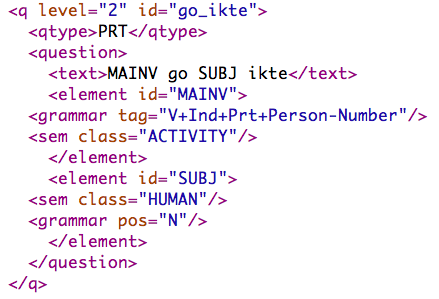
\includegraphics{presentation/img/sentencegenerator.png}}\\
\caption{A question template (MAINV question-particle SUBJ yesterday).}
\label{sentgen}
\end{center}
\end{figure}

In Figure \ref{sentgen} is an example of a question template in which the main verb (MAINV) is fixed to indicative past tense, but the person and number inflection may vary freely. In Figure \ref{vastasent} is the same template is realised as a task in \textit{Vasta}. The user's answer triggers a feedback message about tense of the main verb. 

The question matrices are marked with level, because of a level option offered to the user, e.g. level 1 has only indicative and no past tense. Because of that we have to some extent to fix the inflections in every template, and there are so many as 111 matrix questions. \\

\begin{figure*}[htbp]
\begin{center}
\scalebox{.55}[.55]{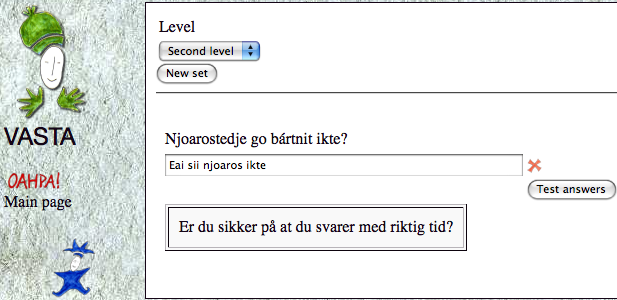
\includegraphics{presentation/img/newvasta.png}}\\
\caption{A generated question and a student's answer in \textit{Vasta}. ("Did the boys use the lasso yesterday?" "No, they do not yesterday.")}
\label{vastasent}
\end{center}
\end{figure*}
 
\subsection{The analysing process} 
Both the question and the answer are analysed with the morphological analyser and then the result is postprocessed to cg3-format with a script.
We use vislcg3 for analysing the user's input. First there is a rule set, which disambiguates the user's input only to a certain extent. The rule set is relaxed compared to the ordinary disambiguator, in order to be able to detect the relevant readings despite of a certain degree of grammatical and orthographic errors in the input. The last part of the file consists of rules for giving feedback to grammatical errors, and rules for navigating to the correct next question or utterance of in the dialogue, due to the user's answer.  

The system question and user answer pairs are merged, and given to the analyser as one text string. The question mark in the question is exchanged for a special symbol ("qst" QDL). We use this symbol, rather than the question mark itself, in order not to introduce a sentence delimiter in the analysis, since we want to refer to the question and the answer separately in the rules (left or right side of the QDL), but also treat the question-answer part as one unit. Many of the constraints are based on the grammar and semantics in the question -- e.g. the tense and person inflection of the verb, the case of NP in the answer and so on. The question itself restricts the possible interpreting of the input. \\


\begin{figure}[htbp]
\begin{center}
\scalebox{.45}[.45]{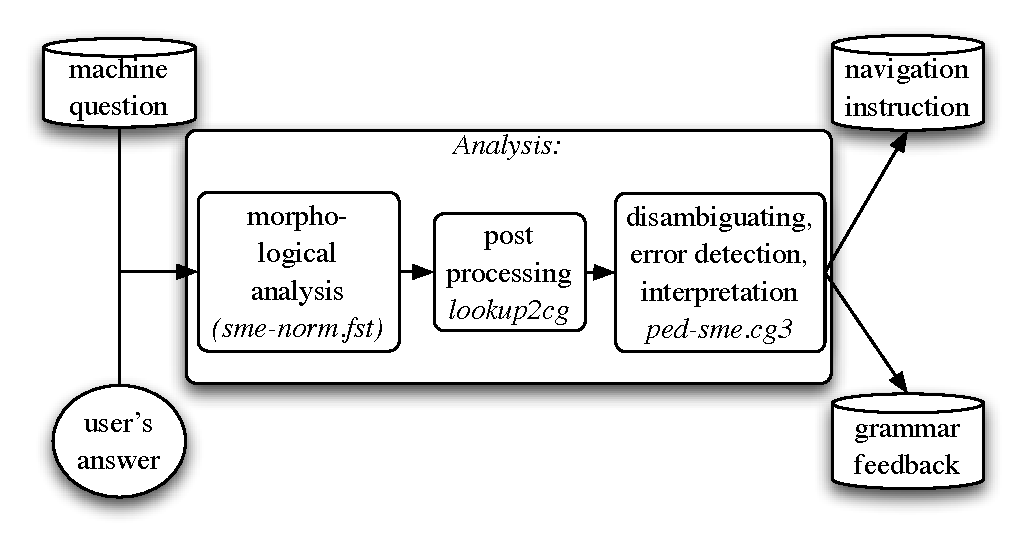
\includegraphics{presentation/img/qa2.pdf}}\\
\caption{Schematical view of the process.}
%\label{nounlex}
\end{center}
\end{figure}


\section{Navigating in the dialogues}
In the \textit{Sahka} dialogues the user may exercise Sámi in a quite natural way and therefore the user's input also needs tags for navigation in the dialogue itself so the user gets correct response to her answer.

The questions in the dialogues are not generated, but written. Every question has its own unique name, so we can link to it from another questions, and it is also possible to make CG-rules for specific questions.  

To show how it works, we can jump into a dialogue in \textit{Sahka}. In Figure \ref{sahka} the setting is visiting a friend who has moved into a new flat, and she needs a helping hand with moving the furniture into the rooms. We have come to the third question and the navigation in the dialogue is due to the answer. In Figure \ref{hivssetanalysis} the analysis assigns two navigation tags to the question-answer pair. The rule for assigning \textit{\&dia-hivsset} is shown in Figure \ref{hivssettag}. ALTERNATIVELY: The rule for assigning the tag \textit{\&dia-hivsset} is: \\
MAP (\&dia-hivsset) TARGET QDL IF \\(0 (where\_place\_TV))\\(*1 ("hivsset") BARRIER Neg OR ROOMS) ; 

This special rule for the question with id \textit{where\_place\_TV} adds the tag if the answer contains \textit{hivsset} (toilet). The barrier is negation verb and words from the semantic set of rooms. \\
 

\begin{figure}[htbp]
\begin{center}
\scalebox{.35}[.35]{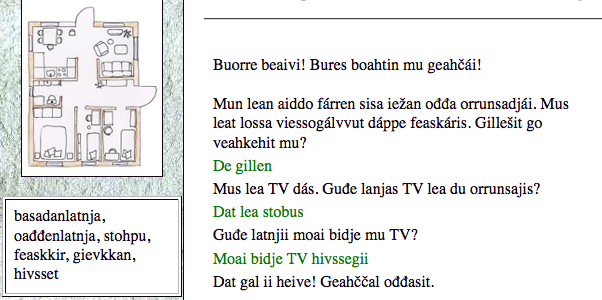
\includegraphics{presentation/img/TVhivssegii.png}}\\
\caption{From \textit{Sahka}. ("In which room should we place the TV?" "We should place it in the toilet." "That is not a good idea. Make a new try.")
}
\label{sahka}
\end{center}
\end{figure}


\begin{figure}[htbp]
\begin{center}
\scalebox{.40}[.40]{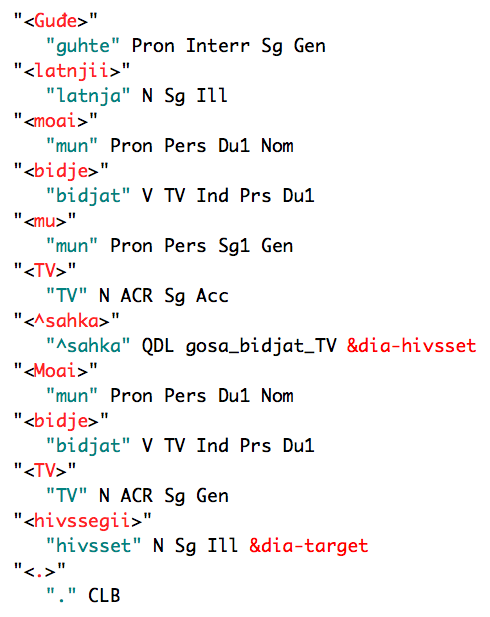
\includegraphics{presentation/img/hivssegiiCGanal.png}}\\
\caption{Assignment of navigation tags is done together with the disambiguation.}
\label{hivssetanalysis}
\end{center}
\end{figure}

\begin{figure}[htbp]
\begin{center}
\scalebox{.45}[.45]{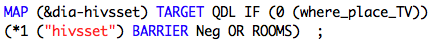
\includegraphics{presentation/img/hivssetrule.png}}\\
\caption{Rule for assignment of navigation tag.}
\label{hivssettag}
\end{center}
\end{figure}



\begin{figure}[htbp]
\begin{center}
\scalebox{.4}[.4]{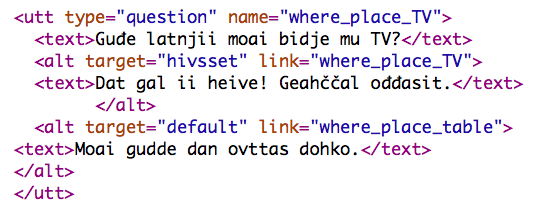
\includegraphics{presentation/img/whereTV.png}}\\
\caption{From the a dialogue file. ("In which room should we place the TV?" Alt. 'toilet': "That is not a good idea. Make a new try." Default: "We carry it there together.") 
}
\label{altlinks}
\end{center}
\end{figure}

The alternative links in the dialogues are connected to the possible tags assigned to the question-answer pair. There will always be a default link in case there will not be any navigation tag. In Figure \ref{altlinks} there are two alternative links for the answers to the question in Figure \ref{hivssetanalysis}. One of them is connected to the \textit{\&dia-hivsset} tag and will give the answer “That is not a good idea. Make a new try.” The other link is default and leads to the next question in the dialogue. 

Many of the rules are general rules. Figure \ref{targettag} is a general target rule for questions, which require an answer in accusative. There are also general rules for tags on whether the answer is interpreted as affirmative or negative, as in Figure \ref{afforneg}. \\
 
\begin{figure}[htbp]
\begin{center}
\scalebox{.3}[.3]{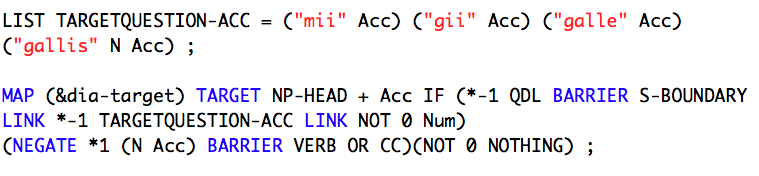
\includegraphics{presentation/img/target_acc.png}}\\
\caption{Assignment of target tag for answer in accusative. 
}
\label{targettag}
\end{center}
\end{figure}

\begin{figure}[htbp]
\begin{center}
\scalebox{.3}[.3]{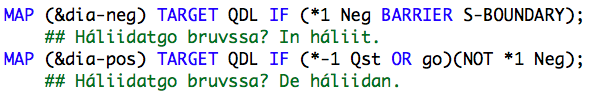
\includegraphics{presentation/img/aff_or_neg_colours.png}}\\
\caption{Tags for affirmative and negative answer. 
}
\label{afforneg}
\end{center}
\end{figure}


There are special tags for information in the user's answer that should be stored. The program is thus able to store simple information such as the user's name, like in Figure \ref{nametag}. The set QMRK consists of question mark, and is given if the name is not in the lexicon, which is quite often with names. There are similar rules and tags for information as place names, car brand and so on, and the information is used of the system in variables in tailored questions or utterances. \\

\begin{figure}[htbp]
\begin{center}
\scalebox{.3}[.3]{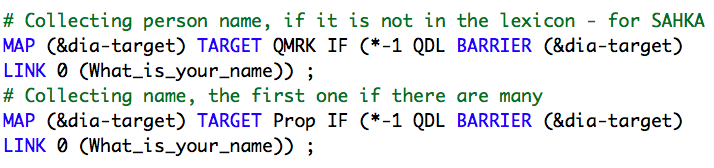
\includegraphics{presentation/img/picking_name_new.png}}\\
\caption{Collecting information from the input for storing.}
\label{nametag}
\end{center}
\end{figure}

To many yes/no-questions the user naturally gives more information. E.g. to the question 'Do you have children?', the user can answer 'Yes, I have two children.' It gives then a bad impression if the next question is 'How many children do you have?'. To prevent that we have a pass-tag for omitting the next question, in this case if the answer contains a numeral, for the question with id \textit{do\_you\_have\_children}, as shown in Figure \ref{omit}.   \\

\begin{figure}[htbp]
\begin{center}
\scalebox{.4}[.4]{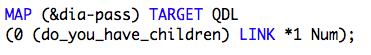
\includegraphics{presentation/img/passchildren.png}}\\
\caption{Rule for assigning tag for omitting the next question.}
\label{omit}
\end{center}
\end{figure}

 
 
Some dialogues are branched according to the user's answer, e.g. in Figure \ref{car} there are different follow-up questions for the answer of 'What kind of car do you have?' If the car brand is in the lexicon, the system picks up the car type and uses it the next question, e.g. 'Is Ford a good car?', and if it is not in the lexicon (it can e.g. be a spelling error or a joke from the user), the next question will be 'Is it a car?'. There is also an alternative link for a negative answer ('Do you want to buy my car?'), and the default leads to a comment which closes this topic. \\

\begin{figure}[htbp]
\begin{center}
\scalebox{.35}[.35]{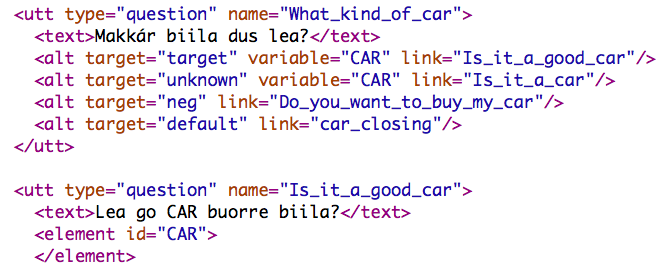
\includegraphics{presentation/img/what_car.png}}\\
\caption{Alternative links due to the answer of 'What car do you have?'.}
\label{car}
\end{center}
\end{figure}

In the same way an answer from the user about her age will induce a tag, which is used to navigate to different branches of the dialogue based on the age of the user, as in Figure \ref{agebranches}. The tag for age is assigned with a regular expression inside a CG-rule, as in Figure \ref{agerule}. \\

\begin{figure}[htbp]
\begin{center}
\scalebox{.4}[.4]{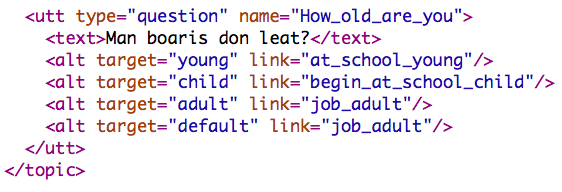
\includegraphics{presentation/img/age_branching.png}}\\
\caption{Alternative branches due to the age of the user. The question is 'How old are you?'.}
\label{agebranches}
\end{center}
\end{figure}

\begin{figure}[htbp]
\begin{center}
\scalebox{.38}[.38]{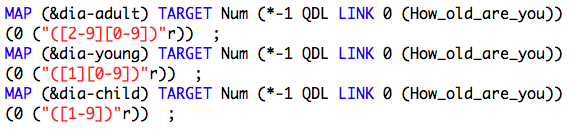
\includegraphics{presentation/img/agerules.png}}\\
\caption{Rules with regular expressions.}
\label{agerule}
\end{center}
\end{figure}

Summary: With help of CG rules one can easily assign tags to the question-answer pair for navigating to the next question or to a special branch of the dialogue according to the containt of the answer. One can also assign a target tag to certain information so the system can collect name, car brand and so on, and use it in a variable in the follow up question.
 
%There are navigation tags for
%\begin{itemize}
%\setlength{\itemsep}{-0.2cm}
%\item affirmative and negative answer 
%\item generell target-tag for the content of the answer
%\item target tags for specific answers to spesific questions
%\item omitting the next question
%\item navigating to a special branch of the dialogue
%\item colllecting information from the input 
%\end{itemize}


\section{Tutorial feedback} \label{tutorial}
The system gives tutorial feedback about grammar errors, both in \textit{Vasta} and in \textit{Sahka}, generated from grammar error tags assigned in the disambiguation analysis. It should be noted that the system uses the grammatical analyser on the fly, exploiting full lexicons. This allows the user's answer to contain any Sámi word, also words that are not restricted to the pedagogical lexicon.

\subsection{Grammar errors} \label{grammarerrors}
In the question in Figure \ref{hivssetloc}, the systems asks “In which room should we place the TV?” The user answers 'Moai bidje TV gievkkanis' ("We should place the TV in the kitchen"), with locative 'gievkkanis' rather than the correct illative 'gievkkanii'. The CG parser disambiguates the input, and the general CG rule in Figure \ref{missingill} adds a grammar-error-tag \textit{\&grm-missing-Ill} to the sentence analysis triggered by the interrogative pronoun followed by a noun in illative, which demands an illative in the answer, when there is not illative or adverb with illative interpretation or negative verb in the answer.  \\ 

\begin{figure}[htbp]
\begin{center}
\scalebox{.4}[.4]{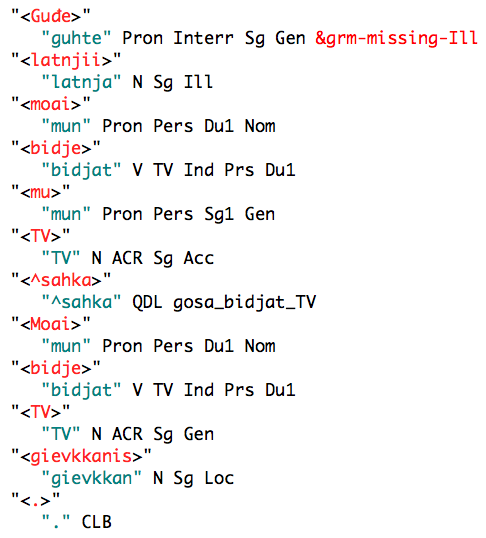
\includegraphics{presentation/img/gievkkanisAnal.png}}\\
\caption{A grammar error tag is assigned. }
\label{hivssetloc}
\end{center}
\end{figure}


\begin{figure}[htbp]
\begin{center}
\scalebox{.4}[.4]{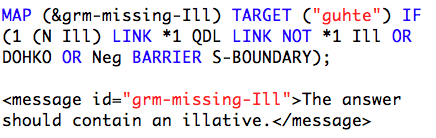
\includegraphics{presentation/img/missingIll.png}}\\
\caption{Rule for assignment of grammar tag.}
\label{missingill}
\end{center}
\end{figure}

One of the pedagogical goals behind the programs is that the user should exercise inflecting the finite verb correctly, so the main rule is that the user has to use a full sentence containing a finite verb. To prevent the user from avoiding the difficult verbs, she has to use the same verb as in the question. The CG-rule in Figure \ref{sameverb} controls the choice of verb for the answer, and uses a regular expression-based tag (a so-called sticky tag). Pro-verbs get a special treatment, so that a question containing a pro-verb will accept any verb in the answer. There is also made exceptions for some auxiliary verbs and for some questions, like the question 'What is your name?' will more naturally be answered without a verb. \\

%For some of the questions in the \textit{Sahka} dialogue the verb requirement is somewhat relaxed. E.g. the question 'What is your name?' will more naturally be answered without a verb.  \\

\begin{figure}[htbp]
\begin{center}
\scalebox{.35}[.35]{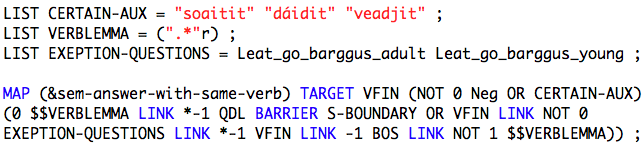
\includegraphics{presentation/img/verblemma.png}}\\
\caption{Rule for giving error tag it there is another finite verb in the answer than in the question.}
\label{sameverb}
\end{center}
\end{figure}


In \textit{Vasta} the pronouns are not allowed to be interpreted inclusively -- \textit{we — you}, not \textit{we — we}, but in \textit{Sahka} they follow the logic of the scenario.

For some questions in the \textit{Sahka}-dialogues which are made for special grammatical training, there are a whole section of rules in the vislcg3 file, for adding specific feedback to the possible errors, e.g. exercise adjective comparision.

The user will get only one feedback at a time, so the error tags are ordered partly a natural progress for error correction, and partly according to the likeliness of the error. First of all the user will get feedback about spelling errors. If there is not agreement between subject and verb, then s/he will get feedback on the verb form, and not on the pronoun, given the assumption that the error is in the verb form rather than in the pronoun.

Grammar errors we have rules for, are
\begin{itemize}
\setlength{\itemsep}{-0.2cm}
%\setlength{\partopsep}{-0.4cm}
\item verbs: finite, infinite, negative form, correct person/tense according to the question
\item case of argument based upon the interrogative 
\item case of argument based upon valency
\item locative vs. illative based upon movement
\item subject/verbal agreement
\item agreement inside NP 
\item numeral expressions: case and number 
\item PP: case of noun, pp based upon the interrogative 
\item time expressions 
\item some special adverbs 
\item particles according to word order
\item comparision of adjectives
\end{itemize}

\subsection{Misspellings}
The biggest problem is the user's misspellings. If the spelling error gives rise to a non-existing word form, then the message to the user is "The word form is not in our lexicon, can it be a spelling error?", which often is not enough help for the user. Here, our program is clearly inferior to a human reader, who would be able to read in a robust way, and detect what the user intended to write. Simulating this ability is not an easy task.
 
Running the feedback through an ordinary speller engine is not a good solution, since the speller will come up with a large number of suggestions, without being able to choose between them. A possible solution would be to run a morphological analysis on the speller suggestions, and let a CG component pick the most likely candidates. The problem is that the current North Sámi speller is made for native speakers and correct mainly typing errors. Needed here is correction of errors due to wrong choice of affices.

We are trying to add rules in the twol-file for typical spelling errors in e.g. place names, in order for the system to give a specific feedback in case of typical misspellings of place names which are in our lexicon. If the place name still is not recognized by the analysator, the feedback is "I haven’t heard about X. Is it a 
place?", and the default link is the next question.

The misspelling can also give rise to another word form of the same lemma. For such cases we make rules based on context. The challenge is to give a feedback according to what the user thinks she has written, because she is probably not aware of the unintended word form. E.g. if the consonant gradation is incorrect in an attempted singular locative, the wordform will be a nominative with possessive suffix Sg3. The learner will probably not know the possessive suffices yet, so it is not use to refer to it. Instead she gets the feedback: "Do you mean locative? Remember consonant gradation." 

A more difficult problem emerges when the spelling error gives rise to an unintended lemma. Then the challenge is to give a feedback according to what the user think she has written. Feedback has to be tailored from what we know about the user’s interlanguage – and we make rules for sets of typical unintended lemmas. Some of them are systematic, e.g. the Sg2 of a verb incorrectly used after the negative verb, will give a ConNeg of a derived verb.  


\subsection{Metacomments}
The way \textit{Sahka} program is created, it makes an illusion of a natural dialogue. But there are some restrictions in the possible input from the user, so the system can analyse the input, and for pedagogical purposes. To remind the user of that, the system sometimes give metacomments to the user, like:
\begin{itemize}
\setlength{\itemsep}{-0.2cm}
\item "Answering \textit{I-don't-know} is too simple. Try again."
\item "Your answer must always contain a finite verb."
\item "You must use one of the words in the wordlist in the left margin."
\item "You have not used the correct adjective. Try again."
\end{itemize}



\section{Evaluation}
The evaluation of \textit{Sahka} and \textit{Vasta} was done when the programs had been available on internet for three months. The user's input and the feedback from the system were logged for the last two weeks of the periode. The system gave 156 tutorial feedbacks. Breaking down the precision numbers on type of feedback, we get the picture as in the Table \ref{ruletypes}. Of 27 errouneous judgements, 16 were due to technical malfunction, 9 to wrong syntactical and 2 to wrong lexical analysis. \\

\begin{table}[htbp]
\begin{tabular}{|l|c|c|c|}
\hline 
\textbf{Rule type}  & \textbf{corr.} & \textbf{wrong}   & \textbf{corr. \% }  \\
\hline 
wrong tense         & 7     & 0     & 100,0     \\ 
wr. V after neg   & 3     & 0     & 100,0     \\ 
no infinite V       & 1     & 0     & 100,0     \\ 
\hline 
orth. error         & 44    & 2     & 95,7      \\
wr. case V-arg  & 26    & 4     & 86,7      \\
no finite verb        & 19    & 4     &  82,6 \\
\hline 
wr. S-V agreem.   & 17    & 8     & 68,0 \\
wrong V choice        & 7     & 4     & 63,6 \\
\hline 
wrong word            & 4     & 4     & 50,0 \\
wr. case after Num  & 1     & 1     & 50,0 \\
\hline
\end{tabular}
\caption{Rule types.}
\label{ruletypes}
\end{table}

As shown in Table \ref{ruletypes} not all of the rule types mentioned in \ref{grammarerrors} have been in use in this period. These rule types have not been used: \\

\begin{itemize}
\setlength{\itemsep}{-0.7cm}
\item agreement inside NP (except for numeral expressions) \\
\item PP: case of noun, pp based of the interrogative  \\
\item time expressions \\
\item particles according to word order \\
\end{itemize}

The reason is probably that the user does not write e.g. complex NP's or complex time expressions or use particles if she is not forced to do it. That is the price of the free input strategy.  \\

Table \ref{errortypes} shows different kinds of error types the system has identified in the user's sentences, \textit{positives}. If it really is an error, then it is a \textit{true positive}, if not, then it is a \textit{negative positive}. It the system has found no error in a sentence, then it is a negative, and they are the same way defined as \textit{true negatives} and \textit{false negative}. \\

\begin{table*}[hbtp]
%\caption{default}
\begin{center}
\begin{tabular}{|l|r|r|r|r||r|r|r|r|r|}
\hline
Error type	& true pos.		& false pos.		& true neg.		& false neg.	& precision	 & recall	& accuracy	& F-ms. \\
\hline
Gramm. error    &   641   &   234   &   769    &   7    &   0,73   &   0,99   &   0,85   &   0,84	  \\
Semant. error       &   805   &   69    &   764    &   12   &   0,92   &   0,99   &   0,95   &   0,95		  \\
Orthogr. error      &   875   &   0     &   776    &   0    &   1      &   1      &   1      &   1					  \\
Other error     &   695   &   180   &   751    &   25   &   0,79   &   0,97   &   0,88   &   0,87	  \\
\hline
  &   3016  &   483   &   3060   &   44   &   0,86   &   0,98   &   0,92   &   0,92			  \\
\hline
\end{tabular}
\caption{Error types.}
\label{errortypes}
\end{center}
%\label{default}
\end{table*}%

We measured \textit{precision} (correctly identified errors/all diagnostised errors), \textit{recall} (correctly identified errors/all errors), and \textit{accuracy} (correct judgements/cases). For the error types we target, precision = 0.85, recall = 0.93, and accuracy = 0.89 (N=277). Better recall than precision indicates that very few errors slip through, at the price of erroneously identifying some correct forms as errors. In this pedagogical setting, a goal for future work is improving precision (avoiding erroneous error flagging).

The high recall compared to the somewhat lower precision indicates that the system is a bit too critical towards the students: It almost never lets through a (targeted) mistake, with the price of flagging some correct answers as errors.
 
\section{Future perspectives}
We have started the work with improving the system.
\begin{enumerate}
%\setlength{\itemsep}{-0.2cm}
\item Something. We will implement a separate SOMETHING (SAARA: help), which will function allover in all dialogues, so one does not have to add this alternative link separately to every question. This makes it possible for the user to quit the dialogue in a proper way by using the verb "heaitit" (= to quit) and then the system navigates to the closing utterance of the dialogue. 
\item Speller. Because the misspellings are the biggest problem for the users, we will implement a speller. We will give relevant suggestions to the user by analysing the list of suggestions according to the context with CG, and also implement weighted lexical transducers, see \cite{Linden:09}. For the waiting we will use the pedagogical lexicon and the north sámi corpus as a training corpus.
\item Topic option. Today \textit{Vasta} generates questions randomly within each level og grammar difficulty. The log shows that this program is not som popular as the \textit{Sahka}. We are planning to make it more interesting for the users by introducing a topic option as well.
\item Sentence construction from given lemmata. We are also concidering how to force the user to construct more complex phraces and also use more particles, by deciding what lemmata the user should use, as a supplement to the other options. Available on internet is \textit{e-tutor} -- a program for teaching German to foreigners \cite{Heift:01,Heift:02}, at \url{http://e-tutor.org}. e-tutor gives very good feedback to student's errors, but the possible input is restricted so the user gets a number of lemmas from which she is to construct a sentence. In this way the user is forced to also write more complex phraces. Figure \ref{etutor} shows an example from the program.
\item Classroom studies. This will be important in the work with improving the system.
\item Porting the programs to more sámi languages. For Lule Sámi a morphological analyser is available, and we have started making a CG disambiaguater. For South Sámi a morphological analyser will be finished in 2010. 
  \end{enumerate} 
  \vspace{0.7cm}

\begin{figure}[htbp]
\begin{center}
\scalebox{.18}[.18]{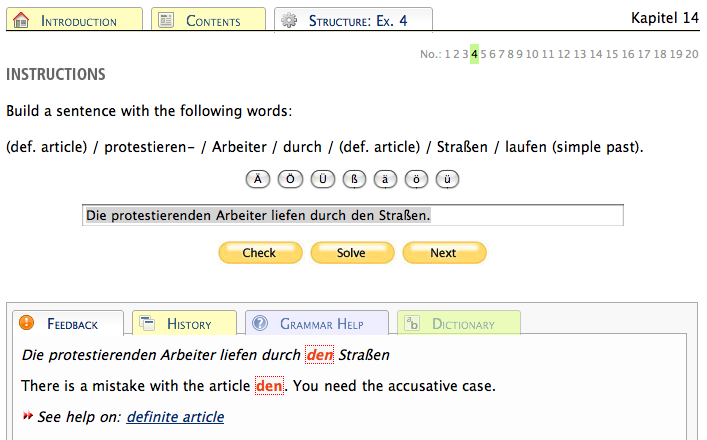
\includegraphics{presentation/img/e-tutor.png}}\\
\caption{An alternative to free input is e-tutor.}
\label{etutor}
\end{center}
\end{figure}

\begin{figure}[htbp]
\begin{center}
\scalebox{.2}[.2]{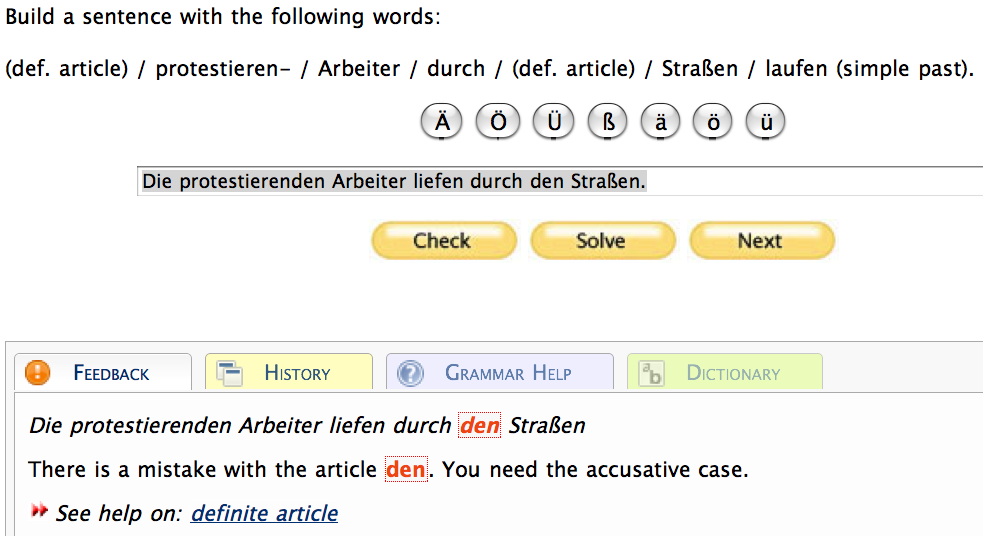
\includegraphics{presentation/img/e-tutor-small.png}}\\
\caption{An alternative to free input is e-tutor.}
\label{etutor}
\end{center}
\end{figure}

\section{Conclusion}
%By using a sloppy version of the CG parser for North Sámi, combined with a set of error-detection rules, we have been able to build a flexible parser-based CALL resource. \\ 
%The precision is not good enough  \\
%We need some kind of speller or a sloppy fst with error tags \\
%"Totally" free input not always the best \\

The paper shows how we have used vislcg3 for pedagogical dialogue systems for Sámi language. Vislcg3 is used in many ways: By relaxing the analysis of the input string, we are able to find errors made by the user, and assign feedback tags to analyse. Secondly, by analysing the semantics in the user's input, and assigning semantic tags to the input, we are able to navigate through the dialogue according to user feedback. And finally, we can assign tag to information in the user's input and use it in the program's questions or utterances.  

The CG formalism has a great potential for use in pedagogical settings.
It is robust enough to handle erroneous data, and at the same time flexible enough to give both general corrections, and corrections targeted at specific words in specific settings.

We have seen that a major problem is spelling errors. Whether CG is able to offer a solution for this problem as well, remains a topic for future research.

\section*{Acknowledgments}
Thanks to the faculty of Humanities at the University of Tromsø, and the Sámi Parliament in Norway, for funding the project. 

\begin{thebibliography}{}

\bibitem[\protect\citename{{Beesley and Karttunen}}2003]{BeesleyKarttunen:03}
{Kenneth R. Beesley and Lauri Karttunen}.
\newblock 2003.
\newblock {\em Finite State Morphology}.
\newblock CSLI publications in Computational Linguistics.
\newblock USA.
%Bick, Eckhard (2003-8). "A Constraint Grammar Based Question-Answering System for Portuguese". In: Fernando Moura Pires & Salvador (eds.) Progress in Artificial Intelligence (Proceedings of EPIA'2003, Beja, Dec. 2003), pp. 414-418. Springer

\bibitem[\protect\citename{Bick}2003]{Bick:03}
{Eckhard Bick}.
\newblock 2003.
\newblock {PaNoLa: Integrating Constraint Grammar and CALL applications for Nordic languages}.
\newblock Holmboe, Henrik (ed.): {\em Nordic Language Technology, Årbog for Nordisk Sprogteknologisk Forskningsprogram 2000-2004}.
\newblock {183--190},
\newblock København: Museum Tusculanums Forlag.

\bibitem[\protect\citename{Bick}2005]{Bick:05}
{Eckhard Bick}.
\newblock 2005.
\newblock {Live use of Corpus data and Corpus annotation tools in CALL: Some new developments in VISL}.
\newblock Holmboe, Henrik (ed.): {\em Nordic Language Technology, Årbog for Nordisk Sprogteknologisk Forskningsprogram 2000-2004},
\newblock {171--185}.
\newblock København: Museum Tusculanums Forlag.

%\bibitem[\protect\citename{Bick}2005b]{Bick:05b}
%{Eckhard Bick}.
%\newblock 2005b.
%\newblock {Grammar for Fun: IT-based Grammar Learning with VISL}.
%%\newblock {49--64},
%\newblock Henriksen, Peter Juel (ed.): {\em CALL for the Nordic Languages.}
%\newblock Copenhagen Studies in Language 30:49--64.

%\bibitem[\protect\citename{Gamper and Knapp}2002]{Gamper:02}
%{Johann Gampfer and Judith Knapp}.
%\newblock 2001.
%\newblock {A review of intelligent CALL systems}.
%\newblock {\em Computer Assisted Language Learning} 
%%\newblock {329--342},
%\newblock {15(4):329--342.}
%%\newblock Routledge.

Lindén, Krister and Tommi Pirinen 2009: Weighted Finite-State Morphological Analysis of Finnish Compounding with HFST-LEXC. Proceedings of the 17th Nordic Conference of Computational Linguistics. Nealt Proceedings Series 4.

\bibitem[\protect\citename{Linden and Pirinen}2009]{Linden:09}
{Kritser Lindén and Tommi Pirinen}.
\newblock 2009.
\newblock {Weighted Finite-State Morphological Analysis of Finnish Compounding with HFST-LEXC}.
\newblock {\em Proceedings of the 17th Nordic Conference of Computational Linguistics.}.
\newblock Nealt Proceedings Series 4.


\bibitem[\protect\citename{Heift}2001]{Heift:01}
{Trude Heift}.
\newblock 2001.
\newblock {Intelligent Language Tutoring Systems for Grammar Practice}.
\newblock {\em Zeitschrift fur Interkulturellen Fremdsprachenunterricht [Online] }
\newblock {6(2).}



\bibitem[\protect\citename{Heift and Nicholson}2001]{Heift:02}
{Trude Heift and Devlan Nicholson}.
\newblock 2001.
\newblock {Web Delivery of Adaptive and Interactive Language Tutoring}.
%\newblock {310--325},
\newblock {\em International Journal of Artificial Intelligence in Education}
\newblock {12(4):310--325.}

%\bibitem[\protect\citename{Heift and Schulze}2007]{Heift:07}
%{Trude Heift and Mathias Schulze}.
%\newblock 2007.
%\newblock {\em Errors and intelligence in computer-assisted language learning: parsers and pedagogues}.
%\newblock Routledge studies in computer-assisted language learning 2. 
%\newblock New York : Routledge.

\bibitem[\protect\citename{Karlsson et. al}1995]{Karlsson:95}
{Fred Karlsson and Atro Voutilainen and Juha Heikkilä and Arto Anttila}.
\newblock 1995.
\newblock {\em Constraint grammar: a language-independent system for parsing unrestricted text}.
\newblock Mouton de Gruyter.


%\bibitem[\protect\citename{Samuelsson and Voutilainen}1997]{SamuelssonVoutilainen:97}
%{Christer Samuelsson and Atro Voutilainen}.
%\newblock 1997.
%\newblock Comparing a Linguistic and a Stochastic Tagger
%\newblock {\em Proceedings of the 35th Annual Meeting of the Association for Computational Linguistics}.
%\newblock {Association for Computational Linguistics},
%\newblock {246--253},
%\newblock {http://www.aclweb.org/anthology/P97-1032}


%\bibitem[\protect\citename{{Trosterud}}2007]{Trosterud:07}
%{Trond Trosterud}.
%\newblock 2007.
%\newblock {\em Language technology for endangered languages: Sámi as a case study}.
%\newblock http://giellatekno.uit.no/background/rvik.pdf
%\newblock University of Tromsø, Norway.

\bibitem[\protect\citename{{visl}}2008]{Visl:08}
{VISL-group}.
\newblock 2008.
\newblock {\em Constraint Grammar}.
\newblock http://beta.visl.sdu.dk/constraint\_grammar.html
%\newblock Institute of Language and Communication (ISK), 
\newblock University of Southern Denmark.


\end{thebibliography}


%\begin{spacing}{1}
%\par
%\bibliographystyle{jmr} %jmr gives the second author with first name first
%\bibliographystyle{jmr}
%\thebibliography{refacl}
%\bibliographystyle{acl}


%\bibdata{refacl}
%\addcontentsline{toc}{section}{References}
%\end{spacing}

	
\end{document}

	
